
	\section{Produkteinsatz}

	\subsection{Beschreibung des Problembereichs}
	Im Folgenden wird der wesentliche Problembereich um eine effiziente, reibungslose, und sichere Gesamtkoordination zu erreichen beschrieben.\\

Zuallererst muss das automatische Fahren im zweidimensionalen Koordinatensystem zu einem angegebenen Zielpunkt fehlerfrei möglich sein.
	Die autonome Steuerung des Roboters muss in der Lage sein, unerwarteten Ereignissen und Hindernissen zu begegnen und diese erfolgreich und unfallfrei zu umfahren. Hindernisse können dabei statisch oder beweglich sein.\\

Als zweite Herausforderung gilt es einen möglichst reibungs- und unterbrechungslosen Batteriebetrieb zu garantieren, um zeitlich vorausschauendes Fahren zu ermöglichen. Im Falle eines niedrigen Batteriestands muss also unverzüglich eine Ladestation angefahren werden um aufzuladen. Außerdem sollen längere Fahrten nicht von Robotern entgegengenommen werden können, deren Akkustand nicht ausreicht um diese Fahrt erfolgreich zu absolvieren.\\

Im dritten Punkt geht es darum, einen Ablauf zu modellieren, für den unglücklichen Fall, dass ein Roboter kaputt gehen sollte. Dies könnte zum Beispiel in einem Unfall passieren.\\

Taxikunden können über eine Serviceapp Anfragen an das System schicken. Das System verwaltet eine Warteschlange, in die neue Aufträge aufgenommen werden. Andererseits können Kunden jederzeit ihre Anfrage abbrechen. Der Server muss die Aufträge in der Warteschlange effizient verteilen, im Speziellen muss eine Priorisierung der Roboter stattfinden, damit jedem Krankentransporter vor dem Taxiservice ein reibungsloser Fahrtverlauf garantiert wird.\\

Die Roboter müssen unter bestimmten Kriterien wie Nähe zum Ziel und aktuellem Batteriestand vom Server ausgewählt werden, und es gilt einzugrenzen, inwieweit die Kriterien wiederum Einfluss auf die Entscheidung des Servers nehmen.\\

Wenn ein Roboter bei einem Patienten oder einem Kunden angekommen ist, müssen Patient und mögliche Helfende bzw. der Fahrtgast benachrichtigt werden. Außerdem muss das Fahrverhalten bzw. die Geschwindigkeit an einen Transport mit Patienten angepasst werden.\\

An die Punkte anknüpfend wird mit folgenden Annahmen gearbeitet:
\begin{enumerate}
	\item Wir starten das System mit voll geladenen Akkus für jeden Roboter.
	\item Es existiert genau ein Krankenhaus und mindestens ein Roboter.
	\item Die Kommunikation funktioniert zuverlässig, insbesondere kommen alle gesendeten \textit{Messages} auch bei dem Empfänger ungeschädigt an. Dazu nehmen wir auch an, dass die Latenz vernachlässigbar klein ist.
	\item Zur Vereinfachung des Fahrverhalten muss jedes Zielobjekt physisch erreichbar sein. Ziele sind dementsprechend keine Hindernisse, das Gleiche gilt für Ladestationen, und sind prinzipiell mit einer Akkuladung erreichbar.
	\item Der Batterieverbrauch bei Robotern ist in einem linearen Verhältnis zur zurückgelegten Strecke.
	\item Bei den beweglichen Objekten wird davon ausgegangen, dass es sich im Verkehrsbetrieb ausschließlich um andere Roboter handelt.
	Für die unbeweglichen Objekte ist es notwendig, dass ihre Position unveränderlich ist.
	\item Im Falle, dass ein Roboter kaputt geht, wird dieser nach einer endlichen Zeit von einem externen, nicht modellierten Unternehmen repariert und kann von seiner letzten Position aus wieder fahren.
	\item Ein Patient ist immer von Helfenden umgeben, die ermöglichen, dass der Patient auf den Roboter geladen wird, und nach der Verladung diesbezüglich das Krankenhaus benachrichtigen.
	\item Wenn ein Kunde ein Taxi bestellt und dieses ankommt, steigt dieser auch zeitnah ein und nimmt seine Fahrt wahr.
	\item Der Taxikunde schließt nach Ankunft bei seinem Ziel die Taxifahrt ab. Er schickt über die TaxiApp also eine entsprechende Nachricht an das System.
	\item Das System startet in einem initialisierten Zustand und ist sofort für Anfragen bereit.
	\item Es gibt maximal genau so viele Krankenhausaufträge wie Roboter in unserem System.

\end{enumerate}

\pagebreak

		\subsection{Glossar}

		% \begin{description}
		% 	\item[Robot]{Roboter, der sich im 2-Dimensionalen Raum bewegen kann.}
		% 	\item[Server]{Verteilt Aufträge an die Roboter}
		% 	\item[Charger]{Ladestation für den Roboter}
		% 	\item[Destination]{Vom Server verwaltete Ziele, die der Roboter ansteuern kann.}
		% 	\item[Obstacle]{Hindernisse, die der Roboter erkennt und umfährt.}
		% \end{description}

			\begin{tabular}{ l p{10cm} }
		\textbf{Begriff} & \textbf{Erklärung}\\
		Robot & Roboter, der sich im 2-Dimensionalen Raum bewegen kann. Der wird
		als Fahrzeug verwendet und kann Personen transportieren.\\
		Position & Eine Position ist eine Zweidimmensionale Position im Raum,
		also ein Punkt, zu dem der Roboter fahren kann\\
		Task & Ein Task behinhaltet zusätzlich zu einer Position auch eine
		Geschwindigkeit. Fadurch kann der Server dem Roboter mitteilen, ob
		dieser vorsichtig oder schnell zu einer Position fahren
		soll.\\
		Server & Der serve ist eine einzelne, zentrale Instanz, die die Aufträge
		an die Roboter verteilt\\
		Charger & Ladestation für den Roboter\\
		Destination & Ziele die der Roboter ansteuern kann.\\
		Obstacle & Hindernisse, die der Roboter erkennt und umfährt Dies können
		entweder andere Roboter sein, mit denen der Roboter kommunizieren kann
		um eine Priorität festzulegen oder statische Hindernisse der
		Umgebung.\\
		Hospital & Das Krankenhaus, das mit dem System kommuniziert, um die Robots
		für Krankentransporte einzusetzen.
	\end{tabular}



		\subsection{Modell des Problembereichs}
		Abbildung \ref{fig:2-3-modell-problembereich} zeigt ein Klassendiagramm, welches das Modell des Problembereichs grafisch darstellt.
		\begin{figure}[H]
			\centering
			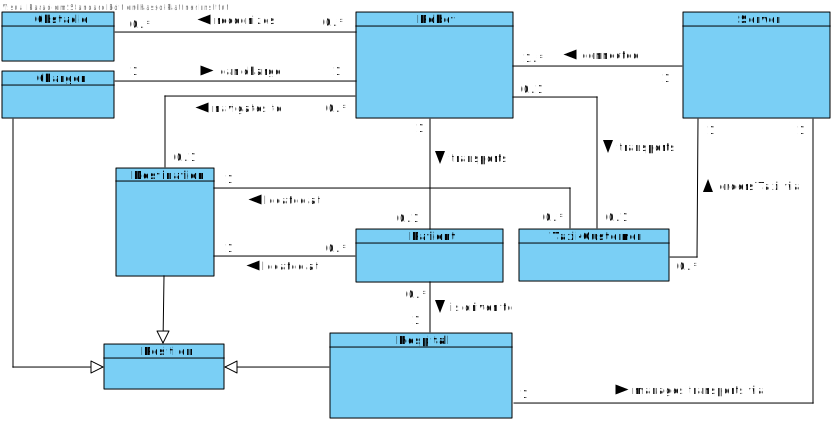
\includegraphics[width=1.0\textwidth]{img/1-Analyse-2}
			\caption{Klassendiagramm des Problembereichs}
			\label{fig:2-3-modell-problembereich}
		\end{figure}

		\subsection{Beschreibung der Geschäftsprozesse}

			\subsubsection{Beschreibung zu 1: Choose Robot}

			\begin{table}[H]
				\centering
				\begin{tabularx}{\textwidth}{|p{3cm}|X|}
				\hline
				\textbf{Auslösendes Ereignis:} & Der Server will für einen bestimmten \emph{Task} den bestmöglichen \emph{Robot} auswählen und diesem den \emph{Task} zuweisen. \\ \hline
				\textbf{Ergebnis:} & Der Server hat einen \emph{Robot} ausgewählt, der für
				diesen  \emph{Task} optimal geeignet ist, und weist diesem den Auftrag zu. \\ \hline
				\textbf{Mitwirkende:} &	Server, Robot \\
				\hline
				\end{tabularx}
				\label{tab:2-4-choose-robot}
			\end{table}

			Abbildung \ref{fig:2-4-choose-robot-aktivitaetendiagramm} zeigt ein Aktivitätendiagramm, welches den Ablauf des Geschäftsprozesses \emph{1: Choose Robot} darstellt.
			\begin{figure}[H]
				\centering
				\includegraphics[width=\textwidth]{img/1-Analyse-3-Choose_Robot}
				\caption{Illustration von \emph{1: Choose Robot} durch Aktivitätendiagramm}
				\label{fig:2-4-choose-robot-aktivitaetendiagramm}
			\end{figure}

			Um den für ein gegebenes Ziel bestmöglichen \emph{Robot} auszuwählen, sendet
			der \emph{Server} zunächst an alle \emph{Robots} eine Anfrage (\emph{request}),
			woraufhin die \emph{Robots} ihre Sensordaten (\emph{sensor data}) auslesen und
			an den \emph{Server} senden. Auf Grundlage dieser Daten wählt der \emph{Server} den
			\emph{Robot} aus, der für die Erfüllung des Zieles am besten geeignet ist.
			Es kann auch vorkommen, dass kein \emph{Robot} geeignet ist, um ein Ziel zu erfüllen.
			Wie die Sensordaten und der Algorithmus zur Wahl des optimalen \emph{Robots} konkret definiert sind, ist eine Entwurfsentscheidung.

			\subsubsection{Beschreibung zu 2: Drive to Destination}

			\begin{table}[H]
				\centering
				\begin{tabularx}{\textwidth}{|p{3cm}|X|}
				\hline
				\textbf{Auslösendes Ereignis:} & Ein \emph{Robot} hat eine \emph{Destination} erhalten.\\ \hline
				\textbf{Ergebnis:} & Der \emph{Robot} ist unter Umfahrung von womöglichen \emph{Obstacles} zur \emph{Destination} gefahren.\\ \hline
				\textbf{Mitwirkende:} &	Ein einzelner, autonomer \emph{Robot}. \\
				\hline
				\end{tabularx}
				\label{tab:2-4-drive-to-destination}
			\end{table}

			\emph{Aufgrund des in der Analyse nicht näher spezifizierten Ablaufs von \emph{Drive to Destination}
			entfällt hier ein Aktivitätendiagramm.}

			Dieser Prozess wird autonom vom \emph{Robot} ausgeführt.
			Er wird genau dann ausgeführt, wenn der Roboter einen \emph{Task} vom Server erhalten hat, den er erfüllen soll.
			Dabei wird vorher festgelegt, mit welcher Geschwindigkeit der \emph{Robot} die in dem \texttt{Task} enthaltene(n) \emph{Destination(s)} jeweils anfahren soll.
			Damit können bei einem Auftrag vom \emph{Hospital} Patienten schneller erreicht werden und sicher zur Klinik gebracht werden.
			Da der \emph{Robot} an dieser Stelle dem \emph{Server} schon bestätigt hat, dass sein Akkustand für die Ausführung des \emph{Tasks} ausreichend ist,
			ist der einzige Sonderfall, den wir betrachten müssen, dass ein \emph{Obstacle} auf der direkten Linie zwischen \emph{Robot} und \emph{Destination} liegt.
			Dann wird der \emph{Robot} nach Wahl des besten Umweges das \emph{Obstacle} umfahren und wieder die Fahrt zur \emph{Destination} aufnehmen. Wie diese Umfahrung durchgeführt wird, ist eine Entwurfsentscheidung.

			\subsubsection{Beschreibung zu 3: Distribute Order}

			\begin{table}[H]
				\centering
				\begin{tabularx}{\textwidth}{|p{3cm}|X|}
				\hline
				\textbf{Auslösendes Ereignis:} & Ein \emph{User} hat eine neue \emph{Order}, die von dem System bearbeitet werden soll.\\ \hline
				\textbf{Ergebnis:} & Die \emph{Order} wird im System aufgenommen und entweder sofort oder sobald ein \emph{Robot} bereit ist bearbeitet.\\ \hline
				\textbf{Mitwirkende:} &	Ein \emph{User} und der \emph{Server}. \\
				\hline
				\end{tabularx}
				\label{tab:2-4-distribute Order}
			\end{table}

			Abbildung \ref{fig:2-4-distribute-order-aktivitaetendiagramm} zeigt ein Aktivitätendiagramm, welches den Ablauf des Geschäftsprozesses \emph{3: Distribute Order} darstellt.

			Ein \emph{User} hat eine \emph{Order}, die das System bearbeiten soll. Diese \emph{Order} wird dem \emph{Server} mitgeteilt, woraufhin der \emph{Server} einen neuen \emph{Task} erstellt. Dieser wird je nach Verfügbarkeit der \emph{Robots} und Priorität des \emph{Tasks} an einen \emph{Robot} verteilt, oder in die vom \emph{Server} verwaltete Warteliste aufgenommen. Der \emph{User} kann über den Use-Case \texttt{Cancel Order} seine \emph{Order} jederzeit während der Ausführung dieses Geschäftsprozesses zurückziehen.

			\begin{figure}[H]
				\centering
				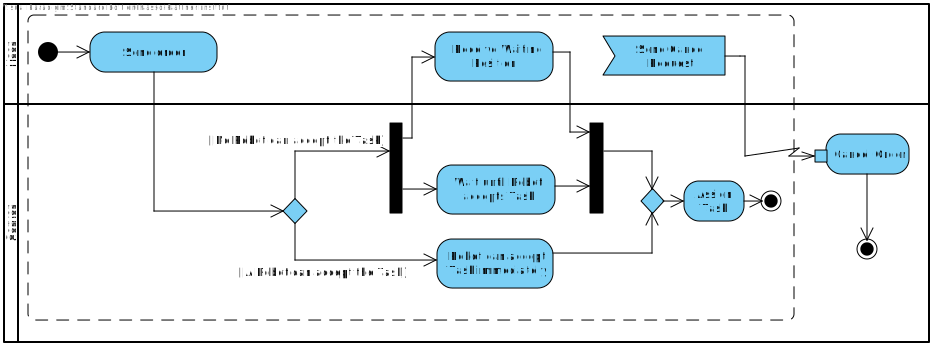
\includegraphics[width=\textwidth]{img/DistributeOrder}
				\caption{Illustration von \emph{3: Distribute Order} durch Aktivitätendiagramm}
				\label{fig:2-4-distribute-order-aktivitaetendiagramm}
			\end{figure}


			\subsubsection{Beschreibung zu 4: Take Customer to Destination}

			\begin{table}[H]
				\centering
				\begin{tabularx}{\textwidth}{|p{3cm}|X|}
				\hline
				\textbf{Auslösendes Ereignis:} & Der \emph{Server} hat einem \emph{Robot} einen neuen \emph{Task} zugeteilt.\\ \hline
				\textbf{Ergebnis:} & Der \emph{Customer} wurde zu seiner \emph{Destination} gebracht.\\ \hline
				\textbf{Mitwirkende:} &	Ein einzelner, autonomer \emph{Robot}. \\
				\hline
				\end{tabularx}
				\label{tab:2-4-take-customer-to-destination}
			\end{table}

			Abbildung \ref{fig:2-4-take-customer-to-destination-aktivitaetendiagramm} zeigt ein Aktivitätendiagramm, welches den Ablauf des Geschäftsprozesses \emph{3: Take Customer to Destination} darstellt.

			Der \emph{Robot} hat eine \emph{Task} vom Server, die er aktuell bearbeiten möchte. Dabei gibt es in dem \emph{Task} gerade eine aktuell zu bearbeitende \emph{Destination}. Der \emph{Robot} fährt diese dann über \texttt{Drive to Destination} an. Im Normalfall wird diese \emph{Destination} dann auch erreicht, und der \emph{Robot} führt die nächste \emph{Destination} in dem \emph{Task} aus. Eine mögliche Unterbrechung in diesem Geschäftsprozess ist, dass der \emph{Robot} einen Unfall hat und dabei kaputt geht - dann fordert er über den Use-Case \texttt{Request Repair} beim Server Hilfe an. Der Geschäftsprozess wird auch unterbrochen, wenn der \emph{Robot} beim ausführen seines aktuellen \emph{Tasks} einen neuen \emph{Task} vom \emph{Server} zugeordnet bekommt. Dies passiert nur, wenn der neue \emph{Task} eine höhere Priorität hat, insbesondere wird immer ein Krankenhaustransport einem Taxitransport vorgezogen.

			\begin{figure}[H]
				\centering
				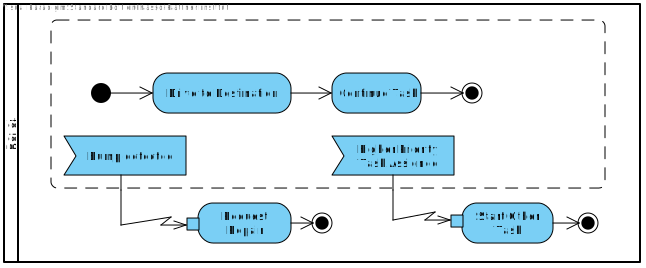
\includegraphics[width=0.8\textwidth]{img/TakeCustomerToDestination}
				\caption{Illustration von \emph{4: Take Customer to Destination} durch Aktivitätendiagramm}
				\label{fig:2-4-take-customer-to-destination-aktivitaetendiagramm}
			\end{figure}
	\pagebreak
